\documentclass[11pt]{article}
\usepackage[top=1in,bottom=1in,left=1in,right=1in]{geometry}                % See geometry.pdf to learn the layout options. There are lots.
%\geometry{letterpaper}                   % ... or a4paper or a5paper or ... 
%\geometry{landscape}                % Activate for for rotated page geometry
%\usepackage[parfill]{parskip}    % Activate to begin paragraphs with an empty line rather than an indent
\usepackage{graphicx}
\usepackage{amssymb}
\usepackage{epstopdf}
\usepackage{amsmath}
\usepackage{amsthm}
\usepackage{hyperref}
\usepackage{color}
\DeclareGraphicsRule{.tif}{png}{.png}{`convert #1 `dirname #1`/`basename #1 .tif`.png}

\usepackage{fancyhdr}

\pagestyle{fancy}
\fancyhf{}
\rhead{Assignment 2}
\lhead{Vector Certificate Program: Neural Networks and Supervised Learning }
\cfoot{\thepage}

%\input{../../misc/macros.tex}

\newcommand{\firstMoments}{\mathbf{m}}
\newcommand{\secondMoments}{\mathbf{v}}
\newcommand{\timeStep}{t}
\newcommand{\gradient}{\mathbf{g}}


\begin{document}

\includegraphics[width=4cm]{vector-logo.png}\newline

\section*{\bf Assignment 2: Model-Agnostic Meta-Learning }


%{\bf Due date:} Nov.~14, 2019 \\

\noindent {\bf Submission:} Submit two files through Classroom: your code file maml-univariate.py and maml-mnist.py.\newline

\noindent The assignments are individual work. 


\begin{enumerate}
\item {\bf MAML} This question is meant to introduce a modern application of automatic differentiation. Much like gradient-based hyperparameter optimization, it involves treating the gradient descent learning procedure itself as a computation graph, and differentiating through it. While the algorithm would be difficult to implement by hand, it only requires a few extra lines of Autograd code compared to ordinary neural network training.

Suppose you want to train an agent that learns to perform many different but related tasks, such as having a robot arm pick up a variety of objects. The agent, through gaining experience with many such tasks, ought to be able to improve the rate at which it can learn similar tasks. This kind of learning is known as \textbf{learning to learn}, or \textbf{meta-learning}.

This question concerns a meta-learning algorithm called \textbf{Model-Agnostic Meta-Learning (MAML, pronounced ``mammal'')}.\footnote{You'reencouraged to read the original paper here \url{https://arxiv.org/abs/1703.03400}} The idea is that if you choose a good enough set of initial weights for the network, it should be possible to learn a new task in only a few steps of gradient descent. Hence, MAML trains a single, task-generic set of weights, with the meta-objective defined as the loss on any particular task after $K$ steps of gradient descent. ($K$ is a small number, such as 5.) The term ``model-agnostic'' is because MAML assumes pretty much nothing about the model, other than that it's trainable by gradient descent.

We will first consider the setting of simple univariate regression tasks. We will sample a distribution of random univariate regression problems, where the inputs are drawn uniformly from the interval $[-3, 3]$, and the functions are random piecewise constant functions with breaks at the integers. For instance,
\begin{center}
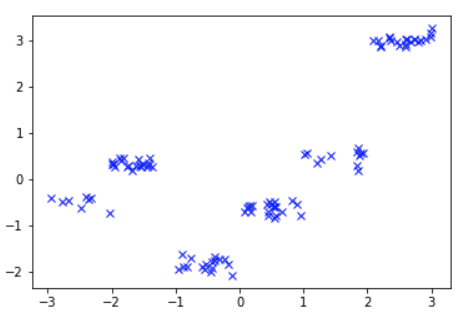
\includegraphics[width=0.3 \textwidth]{data1.png}
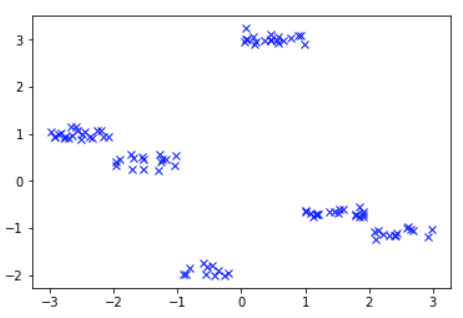
\includegraphics[width=0.3 \textwidth]{data2.png}
\end{center}

It's worth thinking a bit about how the meta-learner might solve this problem. Clearly, 5 iterations would not be enough to train a generic multilayer perceptron (MLP) from scratch. But suppose you initialized the network such that each hidden unit computed a basis function which takes the value 1 on the interval $[k, k+1]$ for some integer $k$, and 0 everywhere else. Then you could fit the function simply by adjusting the weights in the output layer, which is just a linear regression problem, and can therefore be solved pretty quickly. Hence, such a network would be great according to MAML's objective and would be expected to display low values of the objective function of the MAML algorithm. Of course, there are probably other good ways for MAML to solve this problem, and we don't know what it will actually do when we run it.

For the code you will use Autograd, which is a software that can automatically differentiate native Python and Numpy code. The challenging (and hopefully valuable) part is wrapping your head around how the starter code works. This is defined in \verb+maml-univariate.py+. Here are the functions and classes it defines:
\begin{itemize}
  \item \verb+net_predict+: this implements the forward pass for an MLP for the univariate regression problem. The parameters are stored in a Python dict \verb+params+.
  \item \verb+random_init+: initializes the weights to a Gaussian with a small standard deviation.
  \item \verb+ToyDataGen+: This class generates the random piecewise linear functions.
  \item \verb+gd_step+: Performs one step of gradient descent. Note that this function returns a new set of parameters, rather than modifying the arrays that were passed in.
  \item \verb+InnerObjective+: The cost function for \emph{one} regression dataset. This is just mean squared error.
  \item \verb+MetaObjective+: The MAML objective, i.e.~the inner cost after \verb+num_steps+ steps of gradient descent.
  \item \verb+train+: Runs the actual training, i.e.~repeatedly samples random regression datasets and does gradient descent on the meta-objective.
\end{itemize}

Each of these parts requires only a few lines of code, and you should not need to do any new derivation.
\begin{enumerate}
\item  Implement \verb+gd_step+. You should do this by calling \verb+ag.grad+.
\item  Implement \verb+MetaObjective.__call__+. (This is Python syntax for the method that gets called when you call the class instance as if it were a function, i.e.~\verb+meta_obj(params)+.) Your implementation should call \verb+gd_step+.
\item  Finish the implementation of \verb+train+. I.e., sample a random regression dataset, and do a gradient descent step on the meta-objective.
\end{enumerate}

Once you finish the code, calling \verb+train+ will produce a visualization such as the following, where the thinnest line corresponds to the initial parameters learned by MAML, and thicker lines correspond to more steps of SGD:
\begin{center}
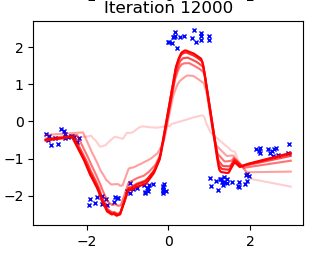
\includegraphics[width=0.3 \textwidth]{gd_example.png}
\end{center}

Observe that your solution will involve calling \verb+gd_step+ on a function which itself calls \verb+gd_step+. Since \verb+gd_step+ calls \verb+ag.grad+, this means you are calling \verb+ag.grad+ on a computation graph which was itself generated by \verb+ag.grad+. Understanding why this happens is an important part of understanding the code.

Submit your code solution as \verb+maml-univariate.py+. You don't need to submit anything else for this question. 

\item {\bf MNIST}

Now that the most important parts of the assignment has been developed, you will extend the MAML algorithm to a more practical dataset of handwritten digits called MNIST. The idea here is to perform meta-learning using an MLP with 2 hidden layers on multiple binary classification tasks. The distribution of tasks corresponds to the classification of uniformly distributed random pairs of MNIST digits in the interval $[0,5]$, e.g. classify 1 vs. 5, 5 vs. 1, 2 vs. 3, 0 vs. 1, 0 vs 2, 2 vs. 0, etc. Note that the solutions you have provided in the first part of the assignment will be used in this section and you won't need to do further modifications to those pieces of code you have already written. 


\begin{enumerate}

    \item Inspect the starter code maml-mnist.py and make sure you understand the distribution of tasks over which the model is going to be trained. This corresponds to understanding the class \verb+ToyDataGen+
    \item Define and initialize appropriate weights of the neural network using a Gaussian distribution with mean zero and standard deviation \verb+ std+ in
    the function \verb+random_init+.
    \item The inner objective of the algorithm will use the cross entropy between the distribution predicted by the neural network and the data. Complete the \verb+InnerObjective+ function with the calculation of the cross entropy. 
    \item Note that in the \verb+train+ function we validate the trained model against the validation set. We compute the classification accuracy of the model before fine tuning, which we anticipate is not going to necessarily be particularly good. However, we anticipate that after fine tuning the
    classification accuracy is going to be high after only a few gradient updates. Your task is to compute the classification accuracy after fine tuning. To do this, you can modify the function \verb+MetaObjective.__call__+ after having internally updated the parameters of the model. 
    \item Print the classification accuracy after fine tuning and try to reason about the difference in the classification accuracy before and after fine tuning.
    \item Train the model with the hyperparameters we have provided. 
    \item Train the model with a number of inner gradient updates  \verb+INNER_STEPS=10+ and observe and discuss  what happens to the meta-objective and the fine tuned classification accuracy.   
    \end{enumerate}



\end{enumerate}



\end{document}
